
\chapter{Design}
\label{ch:methodology}

This chapter presents the design of the project. It is the description of the project's architecture and the project's components.

\section{Baseline design}
\label{sec:baseline_design}

We must design a baseline since we start the project without previous work. The baseline is the starting point of the project. It is the simplest system that we can create to solve the problem. The baseline can then compare the results and improve the system.

The baseline system comprises three main parts: the vehicle recordings, the dataset creation, the model training, and the model testing. The system design is shown in Figure \ref{fig:baseline_system_design}.

\begin{figure}[H]
    \centering
    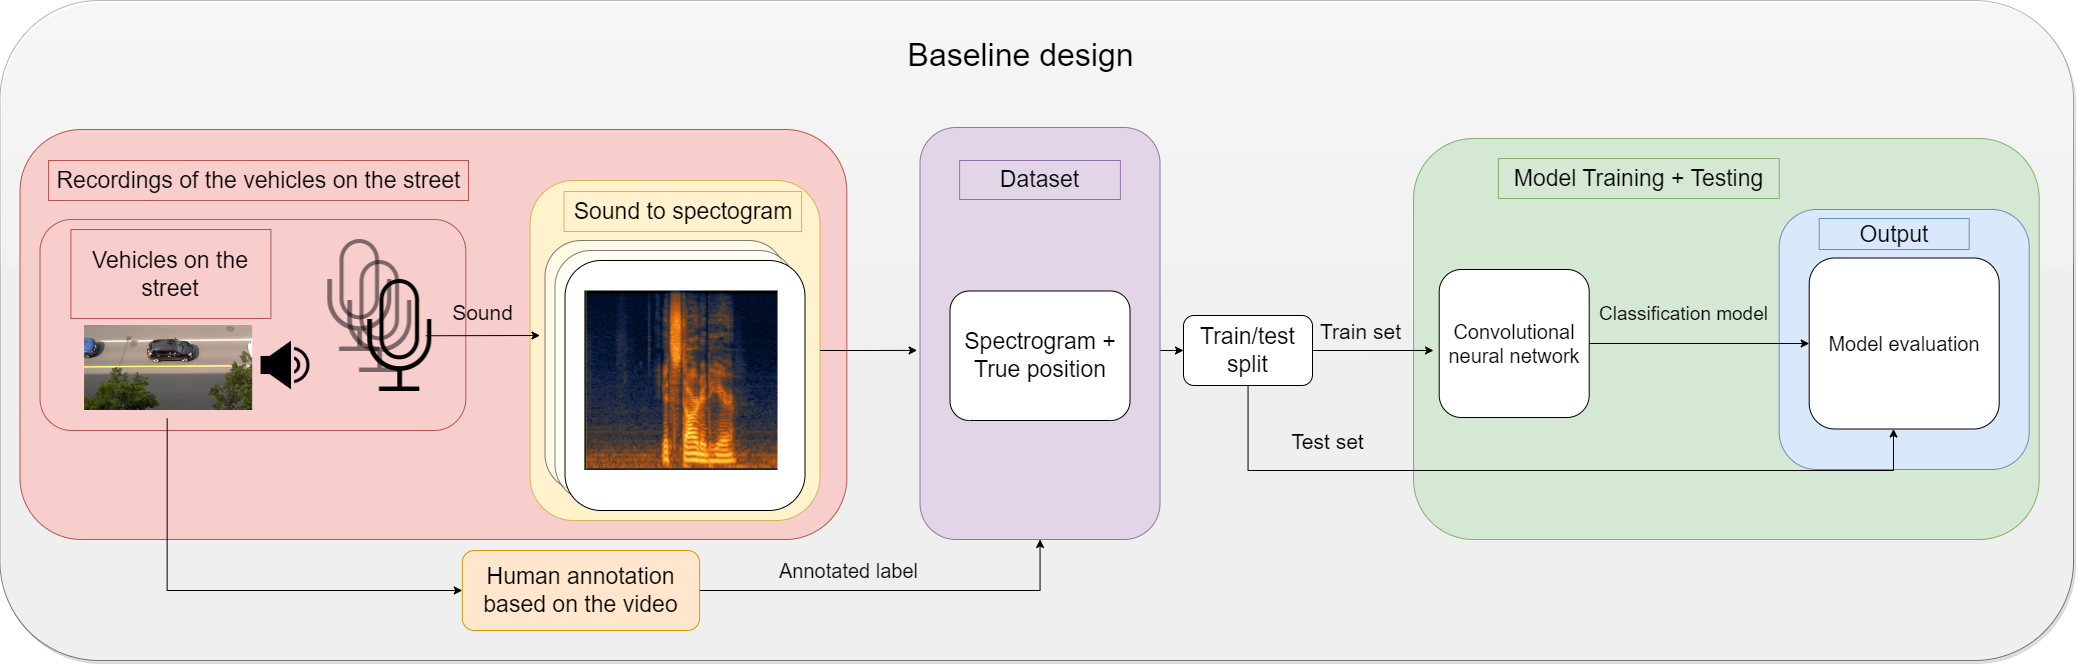
\includegraphics[width=1\textwidth]{../Images/baseline_system_design.drawio.png}
    \caption{Baseline system design}
    \label{fig:baseline_system_design}
\end{figure}

In Figure \ref{fig:baseline_system_design}, the red zone represents the vehicle recordings with multiple microphones and the transformation of the sound into spectrograms. We also record a video to have a ground truth to annotate the dataset. The purple zone represents the dataset creation with the spectrograms as data and the annotations from humans watching the videos as labels. We then split the dataset into a train and a test set. In the green zone, we feed the train set into a neural network to train it to predict the position of the sound source based on the spectrograms. We then test the model on the test set to evaluate its performance with unseen data.

Once we train and evaluate the model, we can use it to predict the position of a sound source based on a new recording. The model can be used in inference to detect the position of a sound source. The inference is shown in Figure \ref{fig:baseline_inference}.

\begin{figure}[H]
    \centering
    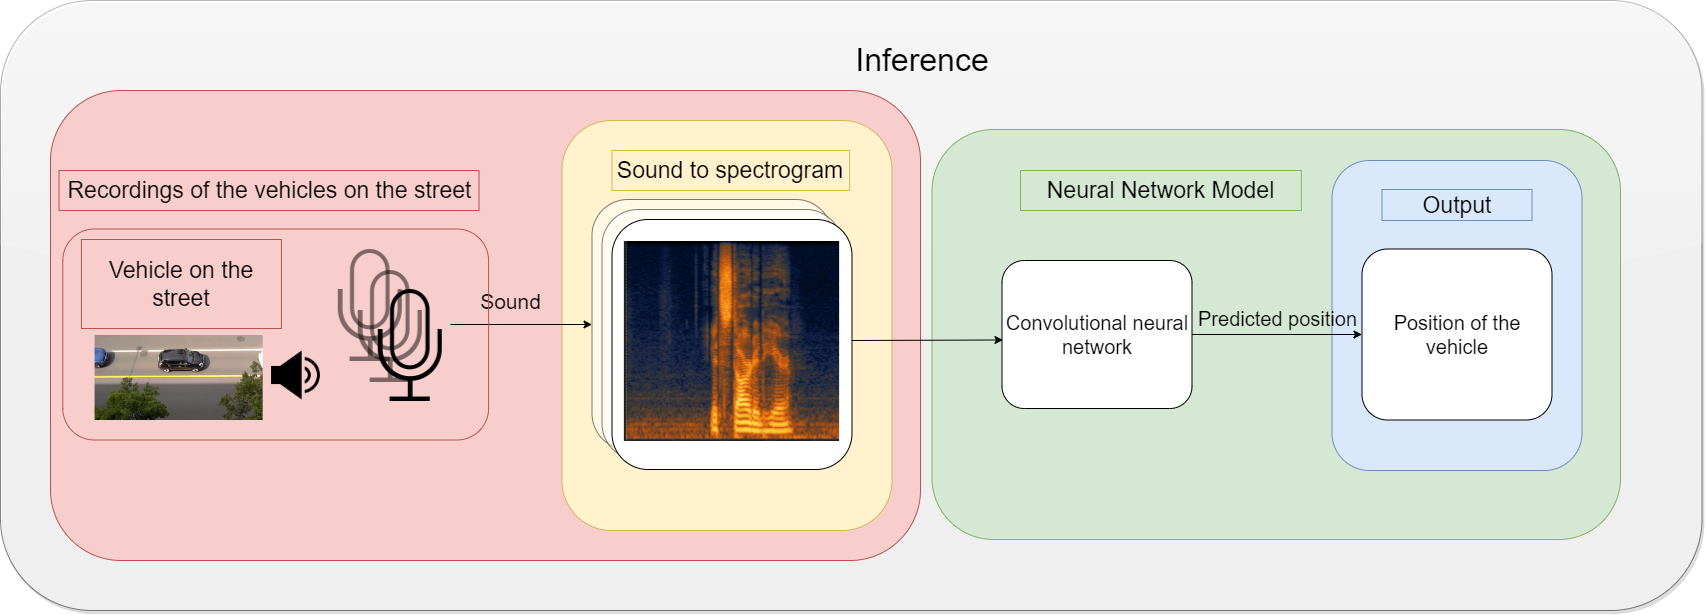
\includegraphics[width=1\textwidth]{../Images/baseline_inference.png}
    \caption{Baseline inference}
    \label{fig:baseline_inference}
\end{figure}

The inference is similar to the training and testing, except that we do not have the ground truth since our model makes the prediction. We only have to do the spectrograms from the recording, and we can feed the spectrograms into the model. The model will then predict the position of the sound source.

We can further develop this idea to incorporate other sound sources for movement tracking in a generalized environment, such as emergency vehicle detection. The baseline is a valuable starting point to develop and test a system that can accurately identify and track sound sources.

\subsection{Vehicle recordings}
\label{sec:vehicle_recordings}
To create the dataset, we must have vehicle recordings with multiple microphones. We place de microphones on the side of the street as shown in Figure \ref{fig:baseline_setup}.

\begin{figure}[H]
    \centering
    \subfloat[\centering Side view]{{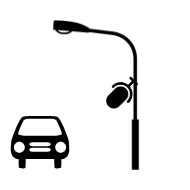
\includegraphics[width=4cm]{../Images/setup_side_view.drawio.png} }}%
    \qquad
    \subfloat[\centering Top down view]{{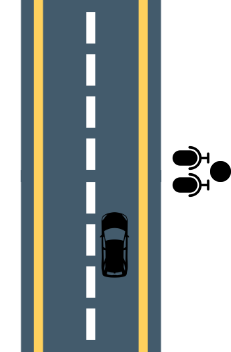
\includegraphics[width=4cm]{../Images/setup_top_down_view.drawio.png} }}%
    \caption{Baseline's microphone setup}
    \label{fig:baseline_setup}
\end{figure}

We also need to record a video of the vehicle to have a ground truth to annotate the dataset. Vehicle recordings are the most crucial part of the baseline. We need to design a system that will allow us to record vehicles from the street and save the data. We designed the system managing the data recording and storage with two microphones, a camera, an embedded system, and a server to store the recordings. This system is shown in Figure \ref{fig:recording_system_design.drawio}.

\begin{figure}[H]
    \centering
    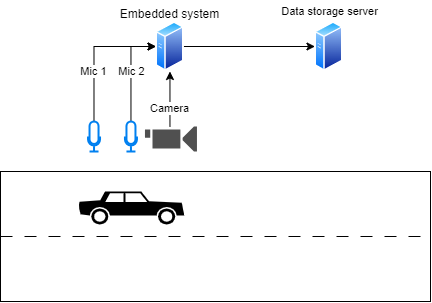
\includegraphics[width=.8\textwidth]{../Images/recording_system_design.drawio.png}
    \caption{Recording system design}
    \label{fig:recording_system_design.drawio}
\end{figure}

Overall, the baseline provides a context to develop further a concept of an accurate sound source localization system for outdoor space.

\subsection{Dataset conception}
\label{sec:dataset_conception}

The dataset is the most crucial part of the baseline. We can determine the dataset's characteristics based on the analysis of the section \ref{sec:datasetsSSL}. The dataset needs to contain the sound recorded by the microphone and the position of the sound source. To simplify the problem, we will use four classes as the main classification challenge in the project. The classes are the following:

\begin{itemize}
    \item  \textit{left\_to\_right}: The vehicle goes from the left to the right of the microphone.
    \item  \textit{right\_to\_left}:  The vehicle goes from the right to the left of the microphone.
    \item  \textit{no\_cars}:  No vehicles pass by the microphone.
    \item  \textit{multiple\_cars}:  Multiple vehicles pass by the microphone.
\end{itemize}

By adding a camera to the system in section \ref{sec:vehicle_recordings}, we can use the image captured by the camera to determine the ground truth of the sound source's position. The camera's position is the same as the microphone's position, and the camera is facing the road. These classes allow the creation of a dataset without precisely recording the vehicle's position. The \textit{no\_cars} and \textit{multiple\_cars} are here to ensure we will have a complete dataset, as with these four classes, we can cover every possible scenario recorded by the microphones and don't need to cherry-pick only the recordings that match our classification system. 

We also used only two classes at the beginning of the project to ensure the concept's functionality when installing the system. These classes are the following:

\begin{itemize}
    \item  \textit{left\_to\_right}:  The vehicle goes from the left to the right of the microphone.
    \item  \textit{right\_to\_left}:  The vehicle goes from the right to the left of the microphone.
\end{itemize}

\subsubsection{Recorded data design}

The input data needs to be an audio signal. Based on the analysis in section \ref{subsec:audio_file_format}, we use the Waveform Audio File Format with pulse-code modulation to represent our audio signal. With this representation, we obtain a vector of floating point numbers representing the audio signal. Since we record multiple channels simultaneously, we can consider the channels as another vector dimension. We can then represent the audio signal as a matrix of floating point numbers.

\section{Convolutional Neural Network design for Sound Source Localization}
\label{sec:cnn_design_for_ssl}

For our baseline, we use a convolutional neural network to predict the position of the sound source. We use a convolutional neural network because, based on the analysis in section \ref{sec:cnn_for_ssl}, it is the most common neural network architecture for image classification and hence for sound source localization. We can use the spectrograms as image input and the convolutional neural network to classify the spectrograms.

The network design is composed of a feature extraction part and a classifier part. The feature extraction part is composed of convolutional layers, ReLU, and pooling layers. The classifier part is composed of fully connected layers. The feature extraction part is used to extract the features from the spectrograms, and the classifier part is used to classify the features extracted. The full architecture is shown in Figure \ref{fig:baseline_feature_extraction}.

\begin{figure}[H]
    \centering
    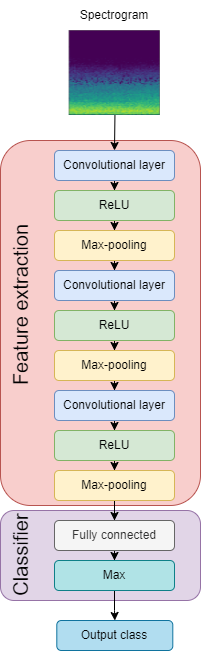
\includegraphics[width=.25\textwidth]{../Images/cnn_architecture_design.drawio.png}
    \caption{Baseline feature extraction}
    \label{fig:baseline_feature_extraction}
\end{figure}

The feature extraction part comprises three blocks of one convolution, one ReLU, and one Max-pooling. The convolutional layers extract the features from the spectrograms. The ReLU layers introduce non-linearity in the network. The pooling layers reduce the dimensionality of the network. The classifier part is composed of one fully connected layer. The fully connected layer classifies the features extracted by the feature extraction part. 

\section{Simulation concept design}

To improve the classification score of the baseline, we need to have more data. Multiple possibilities are available to achieve this goal. We can record more data, but it is time-consuming and expensive. We can also use a simulation to generate new data. In this project, we use a simulation to generate new recordings to add to the training dataset to achieve a better classification score on the baseline. The simulation comprises the same elements in the recording system in section \ref{sec:vehicle_recordings} except we simulate them. The simulation design is shown in Figure \ref{fig:simulation_system_design.drawio}.

\begin{figure}[H]
    \centering
    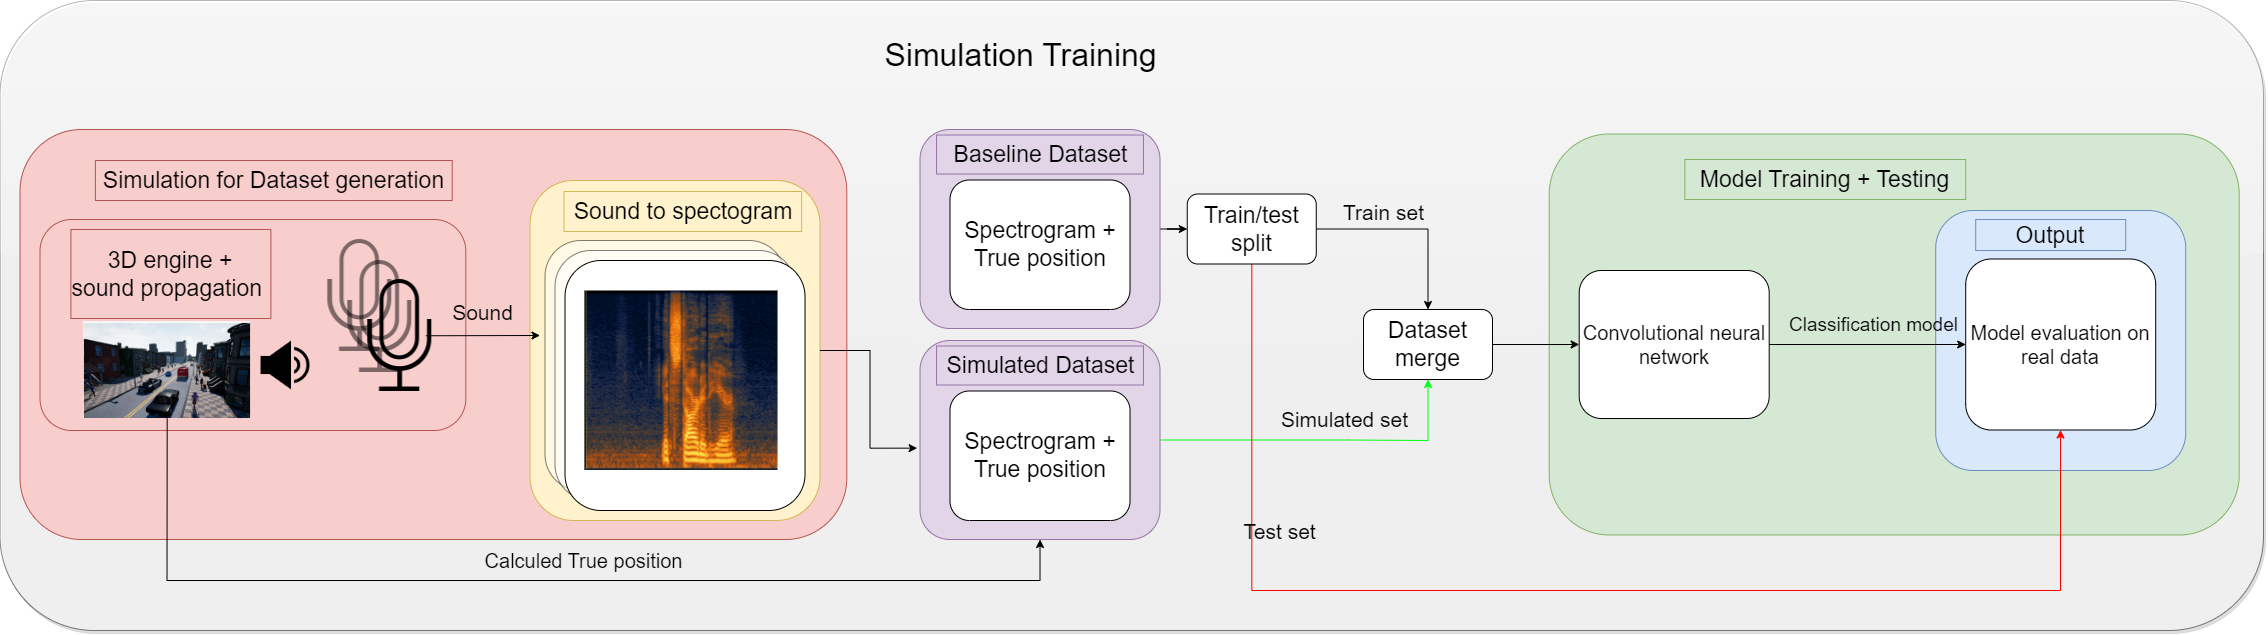
\includegraphics[width=1\textwidth]{../Images/simulation_training_design.drawio.png}
    \caption{Simulation system design for training}
    \label{fig:simulation_system_design.drawio}
\end{figure}

There are differences with the baseline system. The main one is that we generate the data in a simulation. The second is that there is no need to annotate the dataset since we know the position of the sound source in the simulation, and we can deduce the position of the sound directly from the simulation. The last one is that we add the dataset generated by the simulation to the trainset of the baseline but not to the test set. This allows us to understand better the simulation's impact on the real data classification score.

The main advantages of the simulation are that we can generate as much data as we want. We can generate data for any position of the sound source. The simulation is composed of a vehicle, a microphone, and a camera. Based on the section \ref{sec:dataset_conception}, we want to generate data for the classes \textit{left\_to\_right} and \textit{right\_to\_left}. We can generate data for the class \textit{left\_to\_right} by placing the vehicle on the microphone's left and moving it to the right. We can generate data for the class \textit{right\_to\_left} by placing the vehicle on the right of the microphone and moving it to the left. For \textit{no\_cars} class, we can generate data by not placing the vehicle in the simulation. For the \textit{multiple\_cars} class, we can generate data by placing multiple vehicles in the simulation and moving them in the same direction. 

\subsection{Genrealization aspect of the simulation}

For the simulation to best generalize and better represent real-life data, we need to add randomness to the simulation in multiple ways. 

\paragraph{Random speed}

The vehicle's speed is not constant in real life, and we need to add randomness to the vehicle's speed in the simulation. We can add randomness to the vehicle's speed by varying the speed assigned at the beginning of the simulation. 

\paragraph{Random path}

At the beginning of the simulation, we define multiple points as possible start and end points for the vehicle journey. The vehicle's path is generated by randomly choosing a start and end point. We can then generate the vehicle's path by drawing a straight from the start to the end. This method matches the real-life scenario where the straight road in front of the HEIA-FR building constrains the vehicle's path. 

\paragraph{Random starting time}

The vehicle's arrival time is not constant in real life. We add randomness to the vehicle's starting time in the simulation to match the real-life cases. We achieve it by varying the vehicle's waiting time at the simulation's beginning.

\paragraph{Random engine noise}

We need to assign an engine sound to the vehicle during the simulation for the vehicle to be recorded by the microphone. There are many vehicles in real life, and many different engine noises. We reproduce this by randomly choosing an engine noise at the beginning of the simulation and playing it during the simulation. 

\paragraph{Random background noise}

We add randomness to the background noise by randomly choosing a noise track at the beginning of the simulation and playing it during the simulation.

\subsection{Simulation software design}

The simulation should generate audio data by playing scenarios and recording the sound generated inside it. The comportment should represent the ones analyzed in the section \ref{sec:baseline_analysis}. Based on the observation, the scenarios chosen were the following:

\begin{itemize}
    \item \textbf{No cars}: No cars are present in the simulation. The background noise is played during the simulation.
    \item \textbf{Left to right}: A car is present in the simulation. The car starts on the left of the microphone and moves to the right. The background noise is played during the simulation.
    \item \textbf{Right to left}: A car is present in the simulation. The car starts on the right of the microphone and moves to the left. The background noise is played during the simulation.
    \item \textbf{Multiple cars}: Multiple cars are present in the simulation. The cars start on the left of the microphone and move to the right. The background noise is played during the simulation.
\end{itemize}

\section{Adversarial Attack design}

Based on the analysis in section \ref{sec:adversarial_attacks}, we can use an adversarial attack to fool the model designed in section \ref{sec:cnn_design_for_ssl}. This project uses the Fast Gradient Sign Method (FGSM) to generate adversarial inputs. The FGSM is a white-box attack meaning that we need the model's parameters to generate the adversarial inputs. Once we finish training the model, we can calculate the loss function's gradient concerning the input to find the direction that maximizes the loss function. Once we find the direction, we can add a perturbation multiplied by a value of epsilon to the input to generate the adversarial input. 
Once we generate adversarial inputs, we test them on the model to see how it reacts. We realize the attack on a specific value of epsilon. We can try to attack the model with different epsilon values to see how much noise is needed for the model to fail. We analyzed the results by comparing them with the baseline model's results.

\subsection{Audio reconstruction design}

Realizing the adversarial attack by modifying the spectrogram input is not enough to have a negative impact if we use the model for inference in a real-life scenario. Since the system designed in section \ref{sec:baseline_design} uses microphones as input, we need to transform the adversarial spectrogram back to audio. We can then play the audio on a speaker in front of the baseline system to see if the model still fails after the reconstruction of the audio signal.

\subsection{Adversarial attack protection design}

Once we generate the adversarial audio signal, we must again play it through a speaker and the microphone. We can analyze the adversarial audio signal before the classification and try detecting an attempted attack. We can use a classic CNN to classify the type of sound recorded. We can then use the classification score to detect an attempted attack.